\section{Revisiting When is Heterophily Challenging for GNNs}
\label{sec:complexity}

While many works have focused on designing new GNN models with improved performance under heterophily, few of them have probed whether heterophily persistently presents challenges for GNNs. Some of these works have found that GNNs without the aforementioned heterophilous designs (e.g., SGC~\cite{wu2019simplifying}, GCN~\cite{kipf2016semi}, GAT~\cite{velickovic2018graph}) can exhibit better or equivalent performance to GNNs possessing such designs \emph{on certain datasets}~\cite{ma2021homophily,luan2022revisiting}.
In this section, we first summarize the main findings of these works, 
and show that the complexity of heterophily can be measured based on the distinguishability of the Neighborhood Label Distributions (NLDs).\footnote{In parallel with these studies, \citet{yan2022two} conducted a theoretical analysis of performance degradation in heterophilous networks under the ``non-swapping'' condition. This condition emerges when the neighboring representations for each node are \emph{insufficient} to cause the interchange of node representations from two distinct classes across their separation plane in the latent space. Conversely, the case of ``easy heterophily''~\cite{ma2021homophily,luan2022revisiting} that we address in this section corresponds to the ``swapping'' condition as articulated in \cite{yan2022two}.}
We then highlight two key factors, low-degree nodes and complex compatibility matrices, which deteriorate the distinguishability of the neighborhood label distributions when coupled with heterophily, thus making heterophily a unique challenge for GNNs in most cases. 


\subsection{Improved Measures for Complexity of Heterophily}
\label{sec:complexity-measurements}

While many works measure the level of homophily/heterophily by the ratio of edges that connect nodes with the same class label (e.g., edge homophily in Dfn.~\ref{dfn:homophily-ratio}, node homophily~\cite{Pei2020Geom-GCN}, or class homophily~\cite{lim2021large}), recent works have shown that graphs with high heterophily are not always challenging for GNNs without heterophilous designs. 
Through independent analyses, \citet{ma2021homophily} and \citet{luan2022revisiting} arrive at the conclusion that the complexity of heterophily is closely related to the distinguishability of the neighborhood label distributions, which we define next. 

\begin{definition}[Neighborhood Label Distribution (NLD)]
Given $\mathbf{Y}$ as the label encoding matrix defined in \S\ref{sec:preliminaries} for nodes $\vertexSet$ in graph $\graph$, the neighborhood label distribution of node $v$ is defined as
$\mathbf{D}(v) = \tfrac{1}{|N_1(v)|} \sum_{u \in N_1(v)} \mathbf{Y}_u$, where $\mathbf{Y}_u = \mathrm{onehot}(y_u)$ is the $v$-th row of the label encoding matrix $\mathbf{Y}$.
\end{definition}

We now rephrase the two metrics proposed by \citet{ma2021homophily} and \citet{luan2022revisiting} with the above definition, both of which measure the complexity of heterophily by quantifying the distinguishability of $\mathbf{D}(v)$.

\begin{definition}[Class Neighborhood Similarity (CNS)~\cite{ma2021homophily}] %
The class neighborhood similarity between classes $i, j \in \setY$ is defined as the average cosine similarity between the NLDs $\mathbf{D}(v), \mathbf{D}(u)$ of nodes $v, u$ in class $i$ and $j$, respectively, i.e.,
\begin{equation}
    \label{eq:complexity-CNS}
    S(i, j) = \frac{1}{|\vertexSet_i||\vertexSet_j|}\sum_{v \in \vertexSet_i} \sum_{u \in \vertexSet_j} \mathrm{sim}_{\mathrm{cos}}(\mathbf{D}(v), \mathbf{D}(u)),
\end{equation}
where $\vertexSet_i$ and $\vertexSet_j$ are the sets of nodes with class label $i$ and $j$, and $\mathrm{sim}_{\mathrm{cos}}(\cdot)$ is the function of cosine similarity. 
We refer to the case of $i=j$ as \emph{intra-class neighborhood similarity (intra-CNS)} and the case of $i \neq j$ as \emph{inter-class neighborhood similarity (inter-CNS)}.
\end{definition}

\begin{definition}[Graph Aggregation Homophily~\cite{luan2022revisiting}]
Define the average similarity score of a node $v \in \vertexSet$ to nodes $\vertexSet_i$ with class label $i \in \setY$ as
$g(v, i) = \mathrm{mean}\left(\left\{\mathrm{sim}(\mathbf{D}(v), \mathbf{D}(u)) : v, u \in \vertexSet, y_u = i \right\}\right)$, where $\mathrm{sim}$ is a function (e.g., dot product) that measures the similarity between two neighborhood label distributions.
The graph aggregation homophily is then defined as the ratio of nodes $v \in \vertexSet$ where the neighborhood label distribution $\mathbf{D}(v)$ is more similar for nodes in the same class than for nodes in any other class, i.e.,

\begin{equation}
    \label{eq:complexity-gah}
    h_{\mathrm{agg}} = \frac{1}{|\vertexSet|} 
    \left|\left\{ v \in \vertexSet :
    g(v, y_v)
    \geq 
    \max_{j \neq y_v \in \setY}  g(v, j)
    \right\}\right|.
\end{equation}
\end{definition}
We note that while $h_{\mathrm{agg}}$ measures the \textit{proportion} of nodes with NLD exhibiting \emph{greater} similarity (regardless of the extent) to nodes within the same class compared to nodes from different classes, it does not quantify the \textit{degree of similarity} between NLDs of nodes within the same class or across different classes, which is captured by the CNS metric. Consequently, as we show in our empirical analysis in \S\ref{sec:complexity-experiments}, CNS provides a more comprehensive and accurate assessment of the complexity of heterophily on synthetic datasets, and thus we focus on CNS in our empirical analysis below.


\subsection{Factors Determining the Complexity of Heterophily}
It has been shown that it is possible to have graphs with high level of heterophily but low complexity for GNNs as measured by CNS or aggregation homophily~\cite{ma2021homophily,luan2022revisiting}: when nodes in the same class have strong similarity with respect to neighborhood label distributions, and nodes from different classes have weak or no similarity, GCN models are able to perform well due to the high distinguishability of the neighborhood label distributions, even when the graphs are heterophilous.
These are important findings, but this type of analysis does not provide a complete picture of the complexity of heterophily for GNNs, as the high distinguishability of the class label distributions under heterophily is largely dependent on key graph properties, such as degree distributions and the compatibility matrices that drive the generation of the graph. In this section, we provide a detailed analysis of the above two factors that determine how challenging the data heterophily is for GNNs. 

\subsubsection{Motivating Example: Differences in Synthetic Datasets} 
\label{sec:complexity-motivating-example}

Prior research exploring the impact of heterophily on GNN performance frequently incorporates experiments on synthetic datasets with controlled homophily/heterophily levels~\cite{MixHop,zhu2020beyond,ma2021homophily,luan2022revisiting}. 
In line with this research, in this section we provide a motivating example based on synthetic data that showcases the role of the two factors---namely, degree distribution and compatibility matrices---in characterizing how challenging heterophily is for GNN models.
We analyze the seemingly contradictory observations arising from the results on two distinct synthetic datasets based on the \texttt{Cora} dataset: \texttt{syn-cora}~\cite{zhu2020beyond} and \texttt{necessity-cora}~\cite{ma2021homophily}.

Before diving into the analysis of the factors that affect the complexity of heterophily, we first provide a brief overview on the setup and key results on the two synthetic datasets~\cite{zhu2020beyond,ma2021homophily}.

\paragraph{Data Generation: \texttt{syn-cora} vs.~\texttt{necessity-cora}.} 
While both synthetic datasets are generated based on \texttt{Cora}, their generation processes are largely different. 
The \texttt{syn-cora} dataset~\cite{zhu2020beyond,zhu2021graph} follows a modified preferential attachment process. In this process, the probability of a new node $u$ with class label $c$ to attach to existing node $v$ with class label $c'$ is proportional to: 
(1) the ratio $\mathcal{D}_{c,c'}$ specified in the \emph{underlying} compatibility matrix $\mathcal{D}$, which determines the homophily level in the resulting graph, as empirically measured by the edge homophily ratio $h$ (Dfn.~\ref{dfn:homophily-ratio}) and the compatibility matrix $\mathbf{H}$ (Dfn.~\ref{dfn:compatibility-matrix-empirical}),
and (2) the degree $d_v$ of the existing node $v$.
This process results in a power-law degree distribution in the generated graph. 
On the other hand, \texttt{necessity-cora}~\cite{ma2021homophily} varies the level of homophily by adding heterophilous (cross-label) edges on top of the existing (homophilous) edges in \texttt{Cora}. 
To control the randomness of the added heterophilous edges, \texttt{necessity-cora} adds: 
(1) non-random heterophilous edges based on an \emph{underlying} compatibility matrix $\mathcal{D}$, and 
(2) random edges that do not follow the underlying compatibility matrix $\mathcal{D}$, but are controlled by a noise parameter $\gamma$. 

\begin{figure}
    \centering
    \begin{subfigure}[t]{0.453\textwidth}
        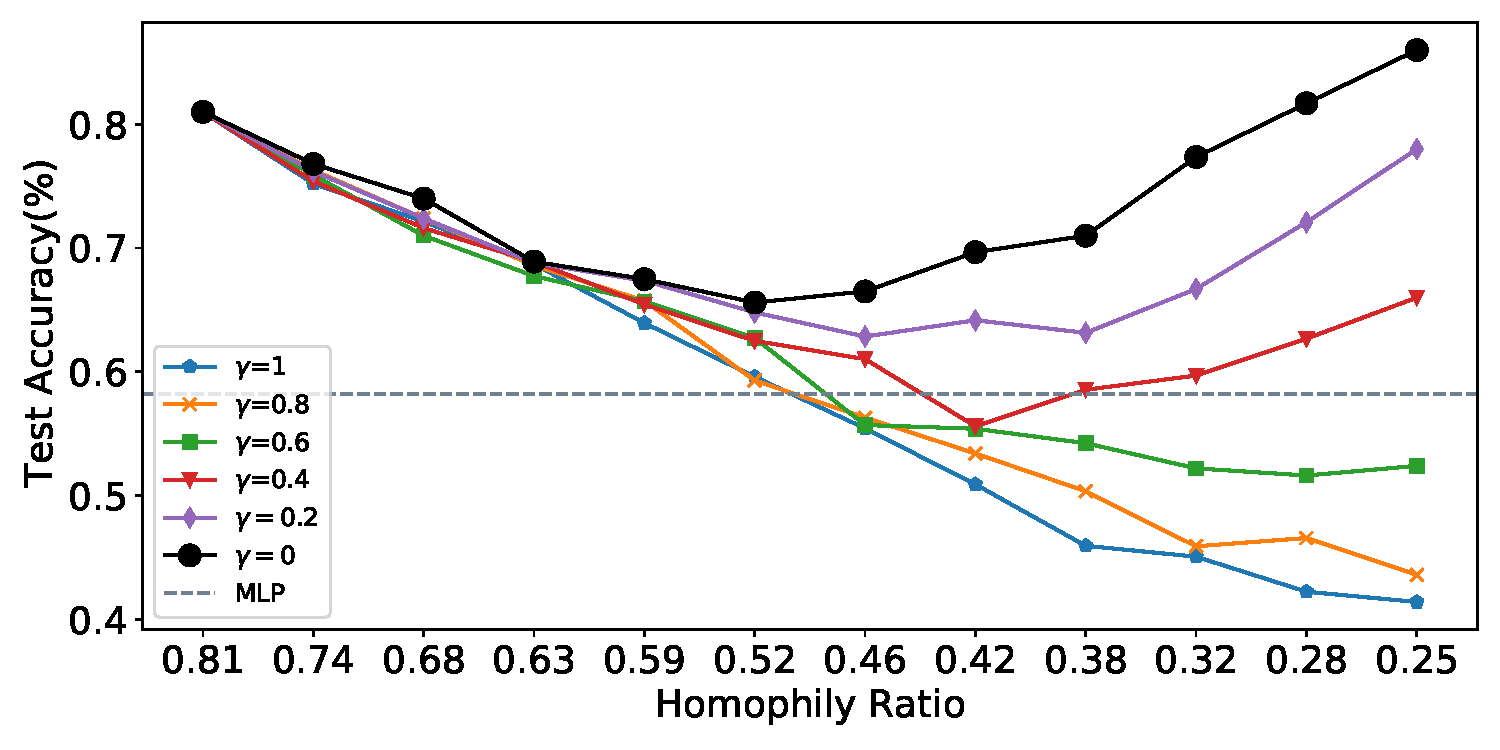
\includegraphics[width=\textwidth]{submissions/Jiong2023/FIG/revisiting-heterophily-GNNs/cora_homo.pdf}
        \caption{Accuracy on \texttt{necessity-cora} %
        under different noise levels $\gamma$. %
        Figure is reproduced from \cite{ma2021homophily}; shared with permission by the authors.}
        \label{fig:revisit-related-observations-necessity-cora}
    \end{subfigure}
    \hspace{0.05\textwidth}
    \begin{subfigure}[t]{0.44\textwidth}
        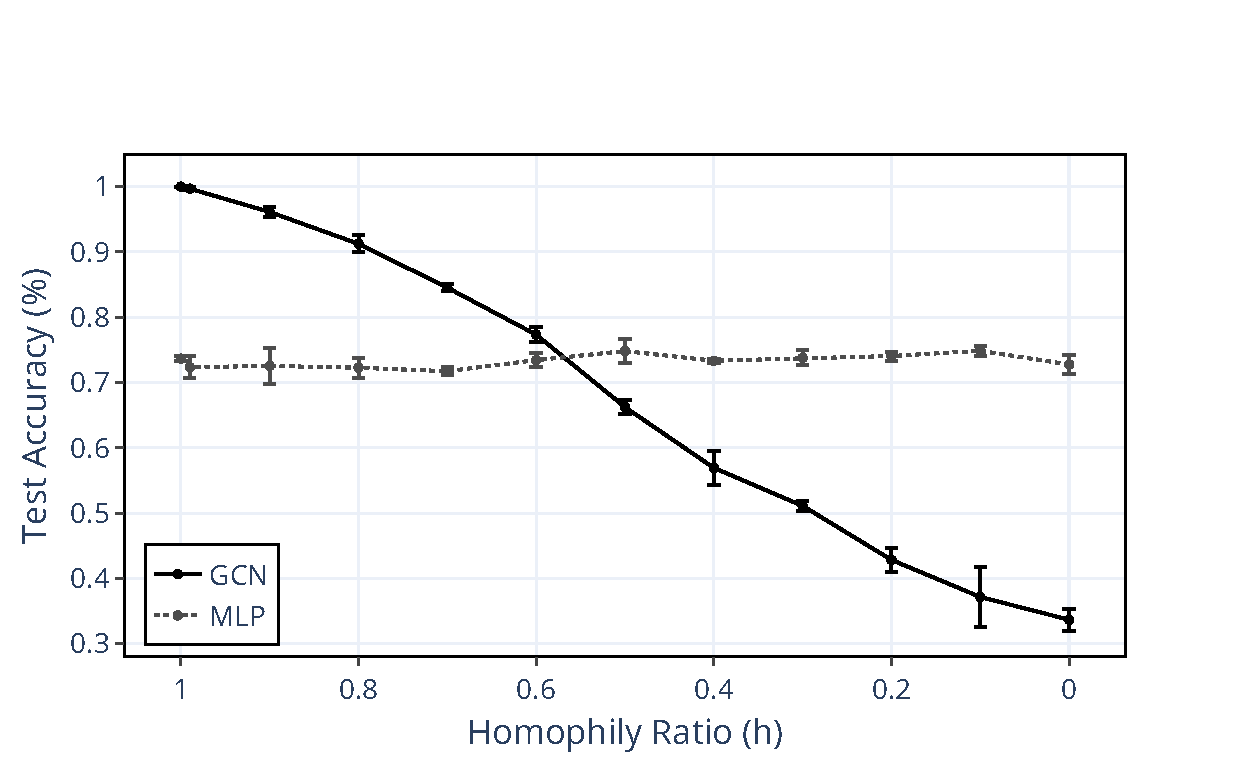
\includegraphics[width=\textwidth]{submissions/Jiong2023/FIG/revisiting-heterophily-GNNs/syn-cora-GCN-results.pdf}
        \caption{Accuracy on \texttt{syn-cora} for  GCN and MLP reported by \cite{zhu2020beyond}. Figure is adapted from \cite{zhu2020beyond}.}
        \label{fig:revisit-related-observations-syn-cora}
    \end{subfigure}
    \caption{Semi-supervised node classification accuracy of GCN and MLP observed in \cite{ma2021homophily} and \cite{zhu2020beyond} on \texttt{necessity-cora} and \texttt{syn-cora}, respectively, under increasing level of \emph{heterophily} (i.e., decrease of the edge homophily ratio $h$). 
    }
    \label{fig:revisit-related-observations}
\end{figure}

\paragraph{Observations: \texttt{syn-cora} vs.~\texttt{necessity-cora}.} 
When the level of heterophily is varied, 
largely different observations are reported on the two sets of synthetic graphs with respect to the GNN performance:
\cite{ma2021homophily} shows that on synthetic graphs with none or few \emph{randomly}-added heterophilous connections (i.e., with the noise parameter $\gamma$ close to 0),
the performance of GCNs can even increase as the level of heterophily in the graph gets stronger (i.e., when the edge homophily ratio $h$ decreases), as shown in Figure~\ref{fig:revisit-related-observations}(\subref{fig:revisit-related-observations-necessity-cora});
on the other hand, \cite{zhu2020beyond} shows that the performance of GCNs significantly decreases 
as the heterophily increases, which we show in Figure~\ref{fig:revisit-related-observations}(\subref{fig:revisit-related-observations-syn-cora}).
As our follow-up analysis below shows, these seemingly contradictory results are due to the different processes used to generate the synthetic graphs, which lead to very different graph properties (i.e., degree distribution, class compatibility matrix); these in turn affect the model performance.
We analyze the effects of the (F1) degree distribution in \S\ref{sec:complexity-factor-degree} and the (F2) compatibility matrix in \S\ref{sec:complexity-factor-compatibility}.

\subsubsection{Factor (F1): Degree Distributions \& Heterophily}
\label{sec:complexity-factor-degree}

In \S\ref{sec:complexity-measurements}, we revisit the findings from recent works~\cite{ma2021homophily,luan2022revisiting} that the complexity of heterophily for GNNs is largely determined by the distinguishability of the Neighborhood Label Distributions (NLDs) of nodes with different class labels. 
Under the generation process of \texttt{necessity-cora} with noise $\gamma=0$ (\S\ref{sec:complexity-motivating-example}), when classes are different $c \neq c'$ and the distributions $\mathcal{D}_{c}$ and $ \mathcal{D}_{c'} $ are distinguishable from each other, one would state that the GCN models can perform well to distinguish the nodes with class label $c$ from the nodes with class label $c'$ from the perspective of NLD distinguishability.



However, we argue that the aforementioned statement ignores the critical factor of degree for each node $v \in \mathcal{V}_c$ that impacts the quality of the samples of the distribution $\mathcal{D}_c$: when all the nodes have sufficiently large degrees, it is expected that $\mathcal{D}_c$ can be recovered well in the node neighborhoods due to sufficient samples of the distributions; however, when many low-degree nodes are present in the graph (which is the case for many real-world graphs, which usually follow power-law degree distributions), $\mathcal{D}_c$ may not be consistently recovered in the neighborhood of the low-degree nodes under heterophily due to the insufficiency of the samples. This affects the intra-class and inter-class similarity of the NLDs in heterophilous settings.


\paragraph{Empirical Analysis.} We can further explain how low-degree nodes affect the intra-class and inter-class distinguishability of the NLD for GCNs under heterophily with a simple empirical analysis: 
Suppose the neighborhood label distributions $\mathcal{D}_c$ and $\mathcal{D}_{c'}$ for two classes $c \neq c'$ are given in the red dashed boxes in Figure~\ref{fig:revisit-degree}.
Following the distributions $\mathcal{D}_c$ and $\mathcal{D}_{c'}$, we randomly generate the NLDs of 200 nodes with degree 2 for both classes $c$ and $c'$; then, we sample the labels of their 2 neighbors, and we visualize a random set of 5 of the 200 synthetic NLDs in Figure~\ref{fig:revisit-degree}(\subref*{fig:revisit-degree-low-heterophily-1})-(\subref*{fig:revisit-degree-low-heterophily-2}), for $\mathcal{D}_c$ and $\mathcal{D}_{c'}$, respectively.
We note that since GCN aggregators additionally consider a self-loop for each node, the NLD observed by GCN models should be considered with self-loops added to the graphs, even when $\mathcal{D}_c$ and $\mathcal{D}_{c'}$ dictate purely heterophilous connections. 
To visualize the contributions of self-loops in the NLDs, we show them in gray in Figure~\ref{fig:revisit-degree}.


\begin{figure}[tp]
    \centering
    \begin{subfigure}[b]{\textwidth}
       \caption*{\textbf{Case 1: Low-degree nodes \& heterophily}}
           \vspace{-0.6cm}
    \end{subfigure}
    \begin{subfigure}[b]{0.47\textwidth}
        \adjincludegraphics[width=\textwidth, trim={0 10.5cm {.5\width} 0}, clip]{submissions/Jiong2023/FIG/revisiting-heterophily-GNNs/dist-hete-low-degree.pdf}
        \caption{\emph{Heterophilous} distribution $\mathcal{D}_c$ of class $c$ (in red box) and 5 sampled NLDs for nodes with degree 2.}
        \label{fig:revisit-degree-low-heterophily-1}
    \end{subfigure}
    \hspace{0.04\textwidth}
    \begin{subfigure}[b]{0.47\textwidth}
        \adjincludegraphics[width=\textwidth, trim={{.5\width} 10.5cm 0 0}, clip]{submissions/Jiong2023/FIG/revisiting-heterophily-GNNs/dist-hete-low-degree.pdf}
        \caption{\emph{Heterophilous} distribution $\mathcal{D}_{c'}$ of another class $c'$ (in red box) and 5 sampled NLDs for nodes with degree 2.}
        \label{fig:revisit-degree-low-heterophily-2}
    \end{subfigure}
    \begin{subfigure}[b]{\textwidth}
       \caption*{\textbf{Case 2: High-degree nodes \& heterophily}}
           \vspace{-0.6cm}
    \end{subfigure}
    \begin{subfigure}[b]{0.47\textwidth}
        \adjincludegraphics[width=\textwidth, trim={0 10.5cm {.5\width} 0}, clip]{submissions/Jiong2023/FIG/revisiting-heterophily-GNNs/dist-hete-high-degree.pdf}
        \caption{\emph{Heterophilous} distribution $\mathcal{D}_c$ of class $c$ (in red box) and 5 sampled NLDs for nodes with degree 10.}
        \label{fig:revisit-degree-high-heterophily-1}
    \end{subfigure}
    \hspace{0.04\textwidth}
    \begin{subfigure}[b]{0.47\textwidth}
        \adjincludegraphics[width=\textwidth, trim={{.5\width} 10.5cm 0 0}, clip]{submissions/Jiong2023/FIG/revisiting-heterophily-GNNs/dist-hete-high-degree.pdf}
        \caption{\emph{Heterophilous} distribution $\mathcal{D}_{c'}$ of another class $c'$ (in red box) and 5 sampled NLDs for nodes with degree 10.}
        \label{fig:revisit-degree-high-heterophily-2}
    \end{subfigure}
    \begin{subfigure}[b]{\textwidth}
       \caption*{\textbf{Case 3: Low-degree nodes \& homophily}}
           \vspace{-0.6cm}
    \end{subfigure}
    \begin{subfigure}[b]{0.47\textwidth}
        \adjincludegraphics[width=\textwidth, trim={0 10.5cm {.5\width} 0}, clip]{submissions/Jiong2023/FIG/revisiting-heterophily-GNNs/dist-homo.pdf}
        \caption{\emph{Homophilous} distribution $\mathcal{D}_c$ of class $c$ (in red box) and 5 sampled NLDs for nodes with degree 2.}
        \label{fig:revisit-degree-low-homophily-1}
    \end{subfigure}
    \hspace{0.04\textwidth}
    \begin{subfigure}[b]{0.47\textwidth}
        \adjincludegraphics[width=\textwidth, trim={{.5\width} 10.5cm 0 0}, clip]{submissions/Jiong2023/FIG/revisiting-heterophily-GNNs/dist-homo.pdf}
        \caption{\emph{Homophilous} distribution $\mathcal{D}_{c'}$ of another class $c'$ (in red box) and 5 sampled NLDs for nodes with degree 2.}
        \label{fig:revisit-degree-low-homophily-2}
    \end{subfigure}
    \caption{{(Factor F1) Degree Distributions}: Per case, we sample 200 NLDs from distribution $\mathcal{D}_c$ (and $\mathcal{D}_{c'}$) for nodes with specific degrees, and visualize 5 sampled NLDs. The gray parts correspond to the contributions of self-loops in the NLDs aggregated by GCN. 
    \textbf{(\subref*{fig:revisit-degree-low-heterophily-1})-(\subref*{fig:revisit-degree-low-heterophily-2}) Case 1:} Low degrees reduce the distinguishability of NLDs: for all synthetic NLDs of $c$ and $c'$, inter-CNS is $S(c, c') = 0.79 \pm 0.17$, with even smaller standard deviation than intra-CNS $S(c, c) = S(c', c') = 0.79 \pm 0.24$.  
    \textbf{(\subref*{fig:revisit-degree-high-heterophily-1})-(\subref*{fig:revisit-degree-high-heterophily-2}) Case 2:} Higher node degrees improve the distinguishability of NLDs: for all synthetic NLDs of $c$ and $c'$, inter-CNS is $S(c, c') = 0.64 \pm 0.15$, which is smaller than the intra-CNS $S(c, c) = S(c', c') = 0.93 \pm 0.09$. 
    \textbf{(e)-(f) Case 3:} Low node degrees matter less under homophily: for all synthetic NLDs of $c$ and $c'$, inter-CNS is $S(c, c') = 0.21 \pm 0.29$, which is significantly smaller than the intra-CNS $S(c, c) = 0.88 \pm 0.15$ and $S(c', c') = 0.91 \pm 0.13$.
    }
    \label{fig:revisit-degree}
\end{figure}



\setlist{leftmargin=*}
\begin{itemize}
\item \textit{Case 1: Low-degree nodes \& heterophily.} 
Figure~\ref{fig:revisit-degree}(\subref*{fig:revisit-degree-low-heterophily-1})-(\subref*{fig:revisit-degree-low-heterophily-2}) show that the existence of low-degree nodes reduces the distinguishability of the NLDs. Specifically, we observe that:
(1)~the intra-class NLDs have a high variance and can be very different from the corresponding ground-truth distributions (even when not considering the self-loops). In fact, the mean and standard deviation of the intra-class pairwise cosine similarity among the 200 synthetic neighborhoods of class $c$ and $c'$ are $0.79\pm 0.24$, where the high standard deviation reflects the strong variance among the sampled neighborhood distributions. (2)~Many of the NLDs from nodes in class $c, c'$ are the same when considering the self-loops, which affects their distinguishability across different classes; the inter-class pairwise cosine similarity for our synthetic neighborhoods of class $c$ and $c'$ is $0.79\pm0.17$ in our analysis, which is the same as the intra-class pairwise similarity with even smaller standard deviation.



\item \textit{Case 2: High-degree nodes \& heterophily.} 
On the other hand, when the node degrees are high, the NLDs are more similar to the underlying distributions $\mathcal{D}_c$ and $\mathcal{D}_{c'}$ (even with self-loops considered) and thus have much smaller variances. In our example, we randomly sampled NLDs of another 200 nodes with degree 10 (instead of 2), and illustrate them for 5 randomly selected nodes in Figure~\ref{fig:revisit-degree}(\subref*{fig:revisit-degree-high-heterophily-1})-(\subref*{fig:revisit-degree-high-heterophily-2}). The mean and standard deviation of the pairwise cosine similarity among the 200 generated neighborhoods of class $c$ and $c'$ are $0.93\pm0.09$, while the inter-class pairwise similarity is only $0.64\pm0.15$. These changes in intra-class and inter-class similarities can also be observed in the sampled distributions shown in Figure~\ref{fig:revisit-degree}(\subref*{fig:revisit-degree-high-heterophily-1})-(\subref*{fig:revisit-degree-high-heterophily-2}).




\item \textit{Case 3: Low- / high-degree nodes \& strong homophily.}
We note that the presence of low-degree nodes does not affect the similarity of NLDs as much in strong homophilous settings as in the heterophilous settings. 
To show this empirically, we similarly generate the neighborhood label distributions of 200 nodes with degrees of 2 for class $c, c'$, but this time with distributions $\mathcal{D}_c$ and $\mathcal{D}_{c'}$ showing strong homophily. 
In Figure~\ref{fig:revisit-degree}(\subref*{fig:revisit-degree-low-homophily-1})-(\subref*{fig:revisit-degree-low-homophily-2}), we observe that, unlike the heterophilous settings, almost all synthetic distributions of nodes from the same class $c$ (or $c'$) are close to the expected distribution $\mathcal{D}_c$ (or $\mathcal{D}_{c'}$); most neighbors (considering self-loops) have the same class label $c$ (or $c'$) as the ego node, even for low-degree nodes. 
Numerically, the intra-class pairwise cosine similarity among the synthetic neighborhoods of class $c$ and $c'$ is $0.88\pm0.15$ and $0.91\pm0.13$, respectively. On the other hand, the inter-class pairwise similarity is $0.21\pm0.29$, which shows good separability. 
This example shows that 
\textbf{the presence of low-degree nodes is a challenge that is more pronounced in heterophilous settings than in homophilous settings.}
\end{itemize}

\begin{wrapfigure}{R}{0.30\textwidth}
    \centering
    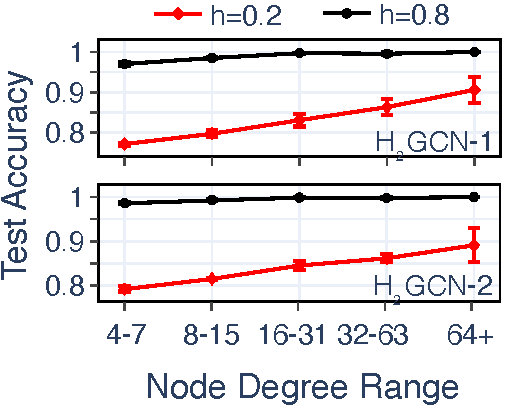
\includegraphics[width=0.28\textwidth]{submissions/Jiong2023/FIG/revisiting-heterophily-GNNs/deg_acc_h2gcn.pdf}
    \caption{\method accuracy per degree range on synthetic heterophilous ($h=0.2$) and homophilous ($h=0.8$) graphs. Figure from \cite{zhu2020beyond}.}
    \label{fig:h2gcn-degree-acc}
\end{wrapfigure}
\paragraph{Summary \& connections to other works.}
From the above analysis, we see that \textbf{the existence of low-degree nodes can lead to weak distinguishability of inter-class NLDs, thus affecting the performance of GCNs}. The significant performance gap between low-degree and high-degree nodes is also observed in \cite{zhu2020beyond},
as shown in Figure~\ref{fig:h2gcn-degree-acc}. 
As a follow-up to our analysis\footnote{These analyses were first made available in the form of a blog post: Zhu, J. and Koutra, D. (2021) Revisiting the problem of heterophily for GNNS. Available at: https://www.jiongzhu.net/revisiting-heterophily-gnns/.}, \citet{ma2021homophily} formalized the effects of node degrees on the distinguishability of NLDs for Contextual Stochastic Block Model (CSBM), and derived a lower bound of node degrees for GCN-style aggregation to improve the distinguishability of NLDs.


\begin{figure}[t]
    \centering
    \begin{subfigure}[t]{0.356\textwidth}
        \adjincludegraphics[width=\textwidth, trim={0.4cm 1cm 2cm 1cm}, clip]{submissions/Jiong2023/FIG/revisiting-heterophily-GNNs/cora-degree.pdf}
        \caption{Degree distribution for \texttt{cora}: it follows a typical power-law degree distribution.}
    \end{subfigure}
    \hspace{0.08\textwidth}
    \begin{subfigure}[t]{0.5\textwidth}
        \adjincludegraphics[width=\textwidth, trim={0.4cm 1cm 2cm 1cm}, clip]{submissions/Jiong2023/FIG/revisiting-heterophily-GNNs/necessity-cora-degree.pdf}
        \caption{Degree distribution of \texttt{necessity-cora}, the cora-based synthetic graphs in \cite{ma2021homophily} with $\gamma=0$ and edge homophily ratio $h\in \{0.077,0.303,0.446,0.584,0.789\}$.}
    \end{subfigure}
    \caption{Degree distributions of \texttt{cora} and \texttt{necessity-cora}. As the level of heterophily increases (i.e., edge homophily ratio $h$ decreases), the degrees for all the nodes increase in \texttt{necessity-cora}, and the degree distributions move further away from the original degree distribution of \texttt{cora}. The shift in degree distribution explains the increase of GCN performance with the level of heterophily for the $\gamma=0$ case in Figure~\ref{fig:revisit-related-observations}(\subref*{fig:revisit-related-observations-necessity-cora}).}
    \label{fig:revisit-cora-necessity-degree}
    \vspace{-0.2cm}
\end{figure}

\paragraph{Revisiting the \texttt{necessity-cora} dataset.} 
The degree distributions of \texttt{necessity-cora} also explain why GCN performance starts to \emph{increase} as the level of homophily $h$ decreases in the range of $h<0.5$ (for noise $\gamma < 0.5$): the \texttt{necessity-cora} graphs with homophily ratio $h<0.5$ have a significantly higher average degree compared to their corresponding base graph \texttt{cora}, as a large amount of edges needs to be added in order to decrease the edge homophily ratio in the (strongly homophilous) base graph. In Figure~\ref{fig:revisit-cora-necessity-degree}, we show the degree distribution of base graph \texttt{cora} in comparison to the degree distributions of the \texttt{necessity-cora} graphs with $\gamma=0$ (i.e., when all the heterophilous edges are added according to the underlying compatibility matrix $\mathcal{D}$, without any randomness) for varying edge homophily ratio $h$. We see that as $h$ decreases, the degrees for all nodes in the graph increase, and the degree distributions move further away from the degree distribution of \texttt{cora}; for the $h=0.077$ instance, even the minimum node degree in the \texttt{necessity-cora} graph has exceeded the degree of most nodes in \texttt{cora}. In our additional empirical analysis (\S\ref{sec:complexity-experiments}), we show that the lack of low-degree nodes is indeed a necessary condition that contributes to the observed high performance of GCNs on \texttt{necessity-cora}.

\subsubsection{Factor (F2): Compatibility Matrices \& Heterophily}
\label{sec:complexity-factor-compatibility}

Another factor that affects the distinguishability of NLDs is the distinguishability of the compatibility matrices for different classes: 
Under the generation process of \texttt{necessity-cora} (\S\ref{sec:complexity-motivating-example}),
when the node degrees are sufficiently high in the generated graphs (Case 2 of \S\ref{sec:complexity-factor-degree}), the NLDs for nodes $v \in \mathcal{V}_c$ are expected to be similar to $\mathcal{D}_c$. 
In this case, the distinguishability of NLDs between nodes in class $c$ and $c'$ mostly depends on the distinguishability of $\mathcal{D}_c$ and $\mathcal{D}_{c'}$, which can also be observed empirically in the compatibility matrices $\mathbf{H}$ of the generated graphs.
In this section, we discuss how complex compatibility patterns in the rows of $\mathbf{H}$ can
reduce the distinguishability of NLDs and contribute to the complexity of heterophily, in addition to (F1) node degrees.



\begin{figure}[t]
    \centering
    \begin{subfigure}[b]{0.31\textwidth}
        \adjincludegraphics[width=\textwidth, trim={0 0 0 {0.13\height}}, clip]{submissions/Jiong2023/FIG/revisiting-heterophily-GNNs/comp-necessity-cora-gamma0.0-h0.165.pdf}
        \caption{Compatibility matrix with $\gamma=0$ and $h=0.16$ in \texttt{necessity-cora}.}
        \label{fig:revisit-comp-matrix-necessity-cora}
    \end{subfigure}
    \hspace{0.02\textwidth}
    \begin{subfigure}[b]{0.31\textwidth}
        \adjincludegraphics[width=\textwidth, trim={0 0 0 {0.13\height}}, clip]{submissions/Jiong2023/FIG/revisiting-heterophily-GNNs/comp-necessity-cora-gamma0.8-h0.163.pdf}
        \caption{Compatibility matrix with $\gamma=0.8$ and $h=0.16$ in \texttt{necessity-cora}.}
    \end{subfigure}
    \hspace{0.02\textwidth}
    \begin{subfigure}[b]{0.31\textwidth}
        \adjincludegraphics[width=\textwidth, trim={0 0 0 {0.13\height}}, clip]{submissions/Jiong2023/FIG/revisiting-heterophily-GNNs/comp-cora-new.pdf}
        \caption{Compatibility matrix of \texttt{cora} with strong homophily.}
        \label{fig:revisit-comp-matrix-cora}
    \end{subfigure}
    \caption{Comparison of compatibility matrices $\matH$ of different synthetic graphs in \texttt{necessity-cora} with homophily ratio $h=0.16$ but different noise ratio $\gamma$, with comparison to the compatibility matrix of \texttt{cora} (the homophilous graph which \texttt{necessity-cora} is based on).}
    \label{fig:revisit-comp-matrices}
\end{figure}

\paragraph{Observations on heterophilous datasets: \texttt{necessity-cora} under different noise levels.} 
The differences in the observed performance of GCN on \texttt{necessity-cora} under different noise levels $\gamma$ (i.e., randomness of the heterophilous edges) in Figure~\ref{fig:revisit-related-observations}(\subref*{fig:revisit-related-observations-necessity-cora}) can be explained by
the differences in the distinguishability of the empirical compatibility matrices $\mathbf{H}$ (and the underlying compatibility matrices $\mathcal{D}$ by extension). In Figure~\ref{fig:revisit-comp-matrices}, we visualize the compatibility matrices of graphs from \texttt{necessity-cora} 
with homophily ratio $h=0.16$, and compare between graphs with noise levels $\gamma=0$ and $\gamma=0.8$:
(1) when $\gamma=0$, the compatibility matrices in \texttt{necessity-cora} are formulated to resemble a ``loop'', where almost all connections for nodes of class $c$ are limited to the two adjacent classes in the ``circle'' of classes (e.g., nodes in Class 2 almost exclusively connect to nodes in Class 1 and 3 in Figure~\ref{fig:revisit-comp-matrices}(\subref*{fig:revisit-comp-matrix-necessity-cora})). 
This ``loop''-pattern helps maintain the high distinguishability of compatibility patterns among different classes, and thus provides an easier node classification problem for GCNs compared to more general heterophilous patterns.
(2) In comparison, when $\gamma=0.8$, the heterophilous connections of class $c$ 
are distributed to all classes $c'\neq c$, and the rows $\mathbf{H}_c$ of the compatibility matrix are less distinct,
which is similar to the case of \texttt{syn-cora} (c.f. Figure~\ref{fig:revisit-dataset-degree-comp}(\subref*{fig:revisit-dataset-degree-comp-syn-cora-comp})).
The high similarity of $\mathbf{H}_c$ among different classes makes it challenging to distinguish different classes from the NLDs even for high-degree nodes, as many heterophilous connections from class $c$ are uniformly distributed to other classes $c'\neq c$. 
This explains the decrease of GCN accuracy under the same homophily level (and degree distribution\footnote{Graphs with the same edge homophily ratio $h$ in \texttt{necessity-cora} also have highly similar degree distributions by extension, since the level of homophily is varied by edge addition.}) in \texttt{necessity-cora} when $\gamma$ increases, as shown in Figure~\ref{fig:revisit-related-observations}(\subref*{fig:revisit-related-observations-necessity-cora}).



\paragraph{Observations on homophilous datasets.} We also note that, echoing the observation in \cite{ma2021homophily}, the \textbf{distinguishability} of the rows in compatibility matrix $\mathbf{H}$ \textbf{is guaranteed for graphs with strong homophily}, as the largest entries in the distributions are concentrated on the diagonal elements of the compatibility matrix $\mathbf{H}$ as shown in Figure~\ref{fig:revisit-comp-matrices}(\subref*{fig:revisit-comp-matrix-cora}). 
\textbf{Thus, the distinguishability of the compatibility matrices is also a challenge specific to heterophilous settings.}

\subsubsection{The Interplay of Degree Distribution, Compatibility Matrices \& NLDs}
\label{sec:complexity-experiments}

In Sections \S\ref{sec:complexity-factor-degree}--\ref{sec:complexity-factor-compatibility}, we discussed two key factors that determine how challenging heterophily is for GNN models. 
Here, we explore the interplay of these factors and NLDs via an empirical study. 
To this end, we construct additional synthetic data with properties complementary to those in \cite{zhu2020beyond,ma2021homophily}. 



\paragraph{Data generation: ``loop''-style schema \& power-law degree distribution.} 
To study the interplay of factors (F1) \& (F2), we generate synthetic graphs which have:
(1) (mostly) %
``loop''-style compatibility matrices (where nodes in each class only connect to nodes in its nearby classes, as if all classes are arranged in a circle), e.g., Figure~\ref{fig:revisit-comp-matrices}(\subref*{fig:revisit-comp-matrix-necessity-cora}).
This schema is similar to that used for \texttt{necessity-cora};
we leverage the same or similar compatibility matrices as specified in \cite{ma2021homophily} in the generation process. (2) the same \emph{power-law} \emph{degree distribution} as \texttt{syn-cora} by following the same modified preferential attachment generation process as in \cite{zhu2020beyond,zhu2021graph}. 

We refer to these synthetic graphs as \texttt{syn-cora-loop}, and consider two variants: \texttt{syn-cora-loop-7} with 7 classes as in \texttt{necessity-cora}, and \texttt{syn-cora-loop-5} with 5 classes as in \texttt{syn-cora}.
In Figure~\ref{fig:revisit-dataset-degree-comp}, we visualize the degree distributions and compatibility matrices of our \texttt{syn-cora-loop} datasets, along with the visualizations for \texttt{necessity-cora} and \texttt{syn-cora}.

\begin{figure}[hbtp]
    \centering
    \begin{subfigure}[b]{0.47\textwidth}
        \adjincludegraphics[width=\textwidth, trim={0 0 0 1.8cm}, clip]{submissions/Jiong2023/FIG/revisiting-heterophily-GNNs/degree-dist-necessity-cora.pdf}
        \caption{Degree distribution of \texttt{necessity-cora} ($\gamma=0$).}
        \label{fig:revisit-dataset-degree-comp-necessity-cora-degree}
    \end{subfigure}
    \hspace{0.04\textwidth}
    \begin{subfigure}[b]{0.47\textwidth}
        \adjincludegraphics[width=\textwidth, trim={0 0 0 1.8cm}, clip]{submissions/Jiong2023/FIG/revisiting-heterophily-GNNs/comp-necessity-cora.pdf}
        \caption{Compatibility matrix of \texttt{necessity-cora} ($\gamma=0$).}
        \label{fig:revisit-dataset-degree-comp-necessity-cora-comp}
    \end{subfigure}
    
    \begin{subfigure}[b]{0.47\textwidth}
        \adjincludegraphics[width=\textwidth, trim={0 0 0 1.6cm}, clip]{submissions/Jiong2023/FIG/revisiting-heterophily-GNNs/degree-dist-necessity-cora-ours-7.pdf}
        \caption{Degree distribution of \texttt{syn-cora-loop-7}.}
    \end{subfigure}
    \hspace{0.04\textwidth}
    \begin{subfigure}[b]{0.47\textwidth}
        \adjincludegraphics[width=\textwidth, trim={0 0 0 1.6cm}, clip]{submissions/Jiong2023/FIG/revisiting-heterophily-GNNs/comp-necessity-cora-ours-7.pdf}
        \caption{Compatibility matrix of \texttt{syn-cora-loop-7}.}
    \end{subfigure}

    \begin{subfigure}[b]{0.47\textwidth}
        \adjincludegraphics[width=\textwidth, trim={0 0 0 1.6cm}, clip]{submissions/Jiong2023/FIG/revisiting-heterophily-GNNs/degree-dist-necessity-cora-ours-5.pdf}
        \caption{Degree distribution of \texttt{syn-cora-loop-5}.}
    \end{subfigure}
    \hspace{0.04\textwidth}
    \begin{subfigure}[b]{0.47\textwidth}
        \adjincludegraphics[width=\textwidth, trim={0 0 0 1.6cm}, clip]{submissions/Jiong2023/FIG/revisiting-heterophily-GNNs/comp-necessity-cora-ours-5.pdf}
        \caption{Compatibility matrix of \texttt{syn-cora-loop-5}.}
    \end{subfigure}

    \begin{subfigure}[b]{0.47\textwidth}
        \adjincludegraphics[width=\textwidth, trim={0 0 0 1.6cm}, clip]{submissions/Jiong2023/FIG/revisiting-heterophily-GNNs/degree-dist-syn-cora.pdf}
        \caption{Degree distribution of \texttt{syn-cora}.}
    \end{subfigure}
    \hspace{0.04\textwidth}
    \begin{subfigure}[b]{0.47\textwidth}
        \adjincludegraphics[width=\textwidth, trim={0 0 0 1.6cm}, clip]{submissions/Jiong2023/FIG/revisiting-heterophily-GNNs/comp-syn-cora.pdf}
        \caption{Compatibility matrix of \texttt{syn-cora}.}
        \label{fig:revisit-dataset-degree-comp-syn-cora-comp}
    \end{subfigure}

    \caption{Synthetic networks used to study the interplay of factors (F1) and (F2).
    \texttt{syn-cora-loop} datasets have the ``loop''-style structure of \texttt{necessity-cora} graphs and the power law degree distribution of the \texttt{syn-cora} graphs.
    }

    \label{fig:revisit-dataset-degree-comp}
\end{figure}




\paragraph{Models.} We assess the influence of degree distributions and compatibility matrices on the performance of three GNN models: \method~\cite{zhu2020beyond}, GCN~\cite{kipf2016semi}, and MLP.
\method represents GNN models that incorporate one or more heterophilous designs as discussed in \S\ref{sec:progress-designs}; we examine two variants of \method, namely \method-1 and \method-2, with one or two layers of aggregation respectively.
In contrast, GCN serves as the GNN baseline model which does not incorporate any heterophilous designs, while MLP functions as the graph-agnostic baseline that does not consider the graph structure.
For GCN, we adopt the same hyperparameter tuning as in \cite{ma2021homophily}, and further tune the dimension of hidden embeddings between 16 and 64.
For \method, we only tune a subset of the hyperparameters that we tune for GCN (16 vs. 112 combinations), which are more hyperparameter combinations than those explored in \cite{zhu2020beyond}.
For each model, we present the mean and standard deviation of the classification accuracy under five runs with different random seeds per dataset.

\paragraph{Data setup.}
Our experiments incorporate four sets of synthetic graphs: \texttt{necessity-cora} provided by \citet{ma2021homophily}, \texttt{syn-cora} from \cite{zhu2020beyond}, and the newly generated \texttt{syn-cora-loop-7} and \texttt{syn-cora-loop-5}.
For \texttt{syn-cora}, we select the graph with homophily level $h=0$; for \texttt{necessity-cora}, we select the graph with noise parameter $\gamma=0$ and $h$ nearest to 0 (i.e., $h=0.03$) as permitted by its generation process. 
We generate \texttt{syn-cora-loop-7} and \texttt{syn-cora-loop-5} with $h=0$. In Table~\ref{tab:revisit-synthetic-results}, we present the statistics for each dataset; the degree distributions and compatibility matrices for all datasets are visualized in Figure~\ref{fig:revisit-dataset-degree-comp}.
For the train/validation/test splits, we utilize the provided splits for \texttt{necessity-cora}~\cite{ma2021homophily}, and create splits for the other datasets using identical sizes as in \texttt{necessity-cora}. Specifically, we randomly select 20 nodes per class for the training set, 500 nodes throughout the graph for the validation set, and allocate the remaining nodes to the test set\footnote{This setup is identical to \cite{kipf2016semi}, but differs from \cite{zhu2020beyond,zhu2021graph} (where Figure~\ref{fig:revisit-related-observations}(\subref*{fig:revisit-related-observations-syn-cora}) was generated), which utilized a larger training set.}.

\begin{table}[t]
\centering
\caption{Dataset statistics and effectiveness of models for node classification. We report the min, median, and max values for the intra-class and inter-CNS, and the mean accuracy $\pm$ standard deviation for each model. The best result for each dataset is highlighted in blue.}
\label{tab:revisit-synthetic-results}
\begin{tabular}{lcccc}
    \toprule
    & \multirow[c]{2}{*}{\shortstack[c]{\textbf{necessity-cora}} } & \multirow[c]{2}{*}{\textbf{syn-cora-loop-7}} & \multirow[c]{2}{*}{\textbf{syn-cora-loop-5}} & \multirow[c]{2}{*}{\textbf{syn-cora}} \\
    \\
    \midrule
    \textbf{\#Nodes} & 2,708 & 2,708 & 1,490 & 1,490 \\
    \textbf{\#Edges} & 132,196 & 5,394 & 2,968 & 2,968 \\
    \textbf{\# Classes} & 7 & 7 & 5 & 5 \\
    \textbf{Edge Hom.} $h$ & 0.03 & 0 & 0 & 0 \\
    \midrule
    \textbf{(F1) High-degree Nodes Only} & \cmark & \xmark & \xmark & \xmark \\
    \textbf{(F2) Compatibility ``Loop''} & \cmark & \cmark & \cmark & \xmark \\
    \textbf{Heterophily Type} & Easy & Challenging & Challenging & Most challenging \\
    \midrule
    \textbf{Agg. Hom.} $h_{\mathrm{agg}}$ & 1.00 & 0.90 & 1.00 & 0.41 \\  %
    \textbf{Intra-CNS} {\small (min/median/max)} & 0.97/0.99/1.00 & 0.79/0.82/0.84 & 0.78/0.80/0.80 & 0.62/0.63/0.64 \\ %
    \textbf{Inter-CNS} {\small (min/median/max)} & 0.00/0.08/0.52 & 0.00/0.31/0.57 & 0.30/0.39/0.47 & 0.53/0.57/0.60 \\ %

    \midrule
    \midrule
    \method-2 & $99.26\pm0.28$ & \cellcolor{blue!20}$88.45\pm1.26$ & \cellcolor{blue!20}$87.98\pm1.49$ & \cellcolor{blue!20}$68.95\pm1.88$ \\
    \method-1 & $93.48\pm0.93$ & $80.85\pm1.69$ & $82.40\pm1.77$ & $66.82\pm2.13$ \\
    GCN & \cellcolor{blue!20}$100.00\pm 0.00$ & $65.10\pm1.80$ & $59.26\pm2.17$ & $27.27\pm1.72$ \\
    MLP & $59.16\pm0.52$ & $58.20\pm2.05$ & $64.16\pm1.61$ & $63.84 \pm2.17$ \\
    \bottomrule
\end{tabular}
\end{table}

\paragraph{GNN performance \& graph properties.} In Table~\ref{tab:revisit-synthetic-results}, we list the performance of each model along with the corresponding properties of the graphs.
We observe the effects of the interplay between low-degree nodes and more complex compatibility matrices to the performance of GNN models when the graphs share similar edge homophily ratio $h$ (0 or as close to 0 as the generation process allows):
\begin{enumerate}[label=(\arabic*),nosep]
\item On \texttt{necessity-cora}, with no low-degree nodes and the simpler ``loop''-style compatibility matrices (Figure~\ref{fig:revisit-dataset-degree-comp}(\subref*{fig:revisit-dataset-degree-comp-necessity-cora-degree})-(\subref*{fig:revisit-dataset-degree-comp-necessity-cora-comp})), models like GCN and \method-2 can achieve near-perfect accuracy.

\item On \texttt{syn-cora-loop} variants, where we keep the ``loop''-style compatibility matrices but modify the degree distributions to follow a power law, we observe 34.90\% to 40.74\% decrease in accuracy for GCN, which falls below the accuracy of \method. As we discussed in \S\ref{sec:complexity-factor-degree}, this heterophilous case is challenging; this is also confirmed by the performance drop for the graph-aware methods, including \method. 

\item On \texttt{syn-cora}, which further strips the ``loop''-style compatibility matrices for heterophilous connections and has more complex connectivity patterns across different classes, the performance of GCN further decreases by 31.99\% and falls much below the performance of the graph-agnostic MLP in this case; though the accuracy of \method variants also decreases significantly in this challenging case, they still outperform MLP in this case.
\end{enumerate}

\paragraph{NLD distinguishability \& graph properties.} The significant changes in the accuracy of GCN can also be explained by the changes in the distinguishability of NLDs caused by different graph properties.
In Table~\ref{tab:revisit-synthetic-results}, we report the Class Neighborhood Similarity (CNS) and Graph Aggregation Homophily $h_{\mathrm{agg}}$ for the all synthetic graphs (as defined in \S\ref{sec:complexity-measurements}, where
we consider self-loops in accordance with GCN aggregation). 
We also visualize the CNS and its standard deviation (following Eq.~\eqref{eq:complexity-CNS}) between pairs of classes on each dataset in Figure~\ref{fig:revisit-dataset-CNS}. 

\begin{figure}[t]
    \centering
    \begin{subfigure}[b]{0.47\textwidth}
        \adjincludegraphics[width=\textwidth, trim={0 0 0 {0.25\height}}, clip]{submissions/Jiong2023/FIG/revisiting-heterophily-GNNs/cross-class-sim-necessity-cora.pdf}
        \caption{CNS of \texttt{necessity-cora} with $\gamma=0$.}
    \end{subfigure}
    \hspace{0.04\textwidth}
    \begin{subfigure}[b]{0.47\textwidth}
        \adjincludegraphics[width=\textwidth, trim={0 0 0 {0.25\height}}, clip]{submissions/Jiong2023/FIG/revisiting-heterophily-GNNs/cross-class-sim-necessity-cora-ours-7.pdf}
        \caption{CNS of \texttt{syn-cora-loop-7}.}
    \end{subfigure}

    \begin{subfigure}[b]{0.47\textwidth}
        \adjincludegraphics[width=\textwidth, trim={0 0 0 {0.25\height}}, clip]{submissions/Jiong2023/FIG/revisiting-heterophily-GNNs/cross-class-sim-necessity-cora-ours-5.pdf}
        \caption{CNS of \texttt{syn-cora-loop-5}.}
    \end{subfigure}
    \hspace{0.04\textwidth}
    \begin{subfigure}[b]{0.47\textwidth}
        \adjincludegraphics[width=\textwidth, trim={0 0 0 {0.25\height}}, clip]{submissions/Jiong2023/FIG/revisiting-heterophily-GNNs/cross-class-sim-syn-cora.pdf}
        \caption{CNS of \texttt{syn-cora}.}
    \end{subfigure}
    \caption{Class neighborhood similarities (CNS) of the synthetic datasets in Table~\ref{tab:revisit-synthetic-results}.}
    \label{fig:revisit-dataset-CNS}
\end{figure}

Based on the intra-class and inter-CNS in Table~\ref{tab:revisit-synthetic-results}, we observe that:
\begin{enumerate}[label=(\arabic*)]
\item With the presence of low-degree nodes, the \texttt{syn-cora-loop} variants have reduced intra-CNS with higher variances compared to \texttt{necessity-cora}, while the inter-CNS also increases, though they share similar ``loop''-style compatibility matrices;
\item The removal of the ``loop'' pattern in the compatibility matrices of \texttt{syn-cora} further reduces the intra-CNS to a level similar to the inter-CNS, which leads to weak distinguishability of the neighborhood label distributions between nodes from different classes. 
These observations explain the decrease of GCN performance observed in our experiments, and show how that the distinguishability of the neighborhood label distributions can depend on other properties like degree distributions and class compatibility matrices in the underlying graphs.
\end{enumerate}

Additionally, we note that while the Aggregation Homophily $h_{\mathrm{agg}}$ is a good indicator of the performance of GCN on \texttt{necessity-cora} and \texttt{syn-cora}, it does not correlate well with the performance changes of GCN on \texttt{syn-cora-loop} variants. 
While $h_{\mathrm{agg}}$ is defined as the \emph{ratio} of nodes with NLD more similar %
to nodes from the same class than nodes from other classes (Eq. \eqref{eq:complexity-gah}), it does not measure the \emph{level of similarity} between the NLDs of nodes from the same or different classes as CNS does. Therefore, we believe that CNS is a more accurate and comprehensive indicator of the complexity of heterophily, as Table~\ref{tab:revisit-synthetic-results} shows. 

\paragraph{Effectiveness of heterophilous GNN designs.} 
With \method as an example that incorporates three heterophilous designs (D1), (D2) and (D3) (discussed in \S\ref{sec:progress-designs}),
we observe that these heterophilous designs can largely improve the performance of GNNs compared to GCNs even when the heterophilous connections do not have the ideal distinguishability in the NLDs as in the \texttt{necessity-cora} ($\gamma=0$) case.
When the distinguishability of NLDs among different classes is low (i.e., when intra-CNS is low and inter-CNS is high), the \method variants largely outperform GCN under heterophilous settings. 
While our experiments focus more on the effects of graph properties to NLD distinguishability and GNN performance and only considered \method as an example for heterophilous GNNs, more comprehensive experiments have been conducted in recent works \cite{platonov2023critical,yan2022two,lim2021large} which support the effectiveness of these heterophilous GNN designs. 

